\documentclass[12pt, twoside]{article}
\usepackage[letterpaper, margin=1in, headsep=0.2in]{geometry}
\setlength{\headheight}{0.6in}
%\usepackage[english]{babel}
\usepackage[utf8]{inputenc}
\usepackage{microtype}
\usepackage{amsmath}
\usepackage{amssymb}
%\usepackage{amsfonts}
\usepackage{siunitx} %units in math. eg 20\milli\meter
\usepackage{yhmath} % for arcs, overparenth command
\usepackage{tikz} %graphics
\usetikzlibrary{quotes, angles}
\usepackage{graphicx} %consider setting \graphicspath{{images/}}
\usepackage{parskip} %no paragraph indent
\usepackage{enumitem}
\usepackage{multicol}
\usepackage{venndiagram}

\usepackage{fancyhdr}
\pagestyle{fancy}
\fancyhf{}
\renewcommand{\headrulewidth}{0pt} % disable the underline of the header
\raggedbottom
\hfuzz=2mm %suppresses overfull box warnings

\usepackage{hyperref}

\fancyhead[LE]{\thepage}
\fancyhead[RO]{\thepage \\ Name: \hspace{4cm} \,\\}
\fancyhead[LO]{BECA / Dr. Huson / Geometry\\*  Unit 9: Dilation \\* 17 March 2023}

\begin{document}

\subsubsection*{9.4 Classwork: Compositions \hfill CCSS.HSG.SRT.B.5}
\begin{enumerate}
\begin{multicols}{2}
[\item A dilation maps $\triangle ABC \rightarrow \triangle DEF$, with $AB=9$, $BC=12$, $AC=6$, and $EF=16$.] \vspace{0.5cm}
  \begin{tikzpicture}[scale=1.4]
    \coordinate [label=above right:$B$](A) at (110:2);
    \coordinate [label=below:$A$](B) at (0, 0);
    \coordinate [label=below:$C$](C) at (-20:1.5);
    \draw [thick] (A)--(B)--(C)--cycle;
    \draw [thick, xshift=2.5cm, yshift=0cm, scale=1.25, rotate=0] 
    (110:2) node[above]{$E$}--
    (0,0) node[below]{$D$}--
    (-20:1.5) node[below]{$F$}--cycle;
    \node at (110:1)[left]{$9$};
    \node at (45:1.3)[left]{$12$};
    \node at (-20:0.75)[below]{$6$};
    \node at (25:3.4)[below]{$16$};
  \end{tikzpicture}\\
  Find the scale factor and missing sides.
  \begin{enumerate}
    \item $\displaystyle k=$ \vspace{0.5cm}
    \item $\displaystyle DE=$ \vspace{0.5cm}
    \item $DF=$ \vspace{0.5cm}
  \end{enumerate}
\end{multicols} \vspace{1cm}
    
\item Dilate the triangle $ABC \rightarrow A'B'C'$ by a factor of $k=1.5$ centered at the origin.
  \begin{multicols}{2}
    \begin{tikzpicture}[scale=.7]
      \draw [help lines] (-4,-4) grid (6,5);
      \draw [thick, ->] (-4.2,0) -- (6.4,0) node [below right] {$x$};
      \draw [thick, ->] (0,-4.2)--(0,5.4) node [left] {$y$};
      \draw [thick] (0,2)node[above left]{$A$}--
        (4,-2)node[below]{$C$}--
        (-2,-2)node[below right]{$B$}--cycle;
    \end{tikzpicture}

    Graph and label the image and complete the table of coordinate mappings.\\[0.5cm]
    $A(0,2) \rightarrow A'(0,3)$ \vspace{3cm}
  \end{multicols}

\item Given $\triangle USA \sim \triangle MEX$ and $m\angle M =60^\circ$, $m\angle E =25^\circ$. Find the remaining angle measures of both triangles.
\begin{flushright}
    \begin{tikzpicture}[scale=0.85]
    \coordinate [label=above left:$S$](A) at (60:3.5);
    \coordinate [label=left:$U$](B) at (0, 0);
    \coordinate [label=below:$A$](C) at (0:1.5);
    \draw [thick] (A)--(B)--(C)--cycle;
    \draw [thick, xshift=5cm, yshift=4cm, scale=1.5, rotate=-120] (60:3.5) node[right]{$E$}--
    (0,0) node[right]{$M$}--
    (0:1.5) node[left]{$X$}--cycle;
  \end{tikzpicture}
\end{flushright}

\newpage
\item A dilation centered at $A$ with a scale factor of $\displaystyle k=2.5$ maps $\triangle ABC \rightarrow \triangle ADE$. Given $AB=9.0$, $AC=12.2$, $DE=18.0$. 
\begin{multicols}{2}
  Find the following side lengths:\\[0.25cm]
  $AD=$\\[1cm]
  $AE=$\\[1cm]
  $BC=$\\
  \begin{flushright}
    \begin{tikzpicture}[scale=0.8]
      \draw [thick]
      (0,0)node[below]{$A$}--
      (0:6)node[below]{$D$}--
      (30:8)node[above]{$E$}--cycle;
      \draw [thick]
      (0:2.4)node[below]{$B$}--
      (30:3.2)node[above left]{$C$};
      \node at (0:1.5)[below]{$9.0$};
      \node at (15:6.75)[right]{$18.0$};
      \node at (35:1.7)[above]{$12.2$};
    \end{tikzpicture}
  \end{flushright}
\end{multicols}

\item Rotate $\triangle ABC$ $180^\circ$ counterclockwise around the origin. Then, dilate $\triangle A'B'C'$ by a factor of $\displaystyle k=\frac{5}{3}$ centered at the origin to produce $\triangle A''B''C''$. Plot and label the two triangles in the graph below.
\begin{center}
  \begin{tikzpicture}[scale=0.8]
    \draw [help lines] (-10,-7) grid (8,6);
    \draw [thick, <->] (-10.4,0) -- (8.4,0) node [right] {$x$};
    \draw [thick, <->] (0,-7.4)--(0,6.4) node [above] {$y$};
    \draw [thick]
      (0,0) node[below right] {$A$}--
      (6,3) node[above right] {$B$}--
      (6,0) node[below] {$C$}--
      cycle;
  \end{tikzpicture}
\end{center}
Would the same triangle result if you dilated first and then rotated? When are rotation and dilation ``commutative'', never, sometimes, always?

\newpage
\item Dilate $\triangle ABC \rightarrow \triangle A'B'C'$ by a factor of $k=\frac{1}{2}$ centered at $(0,0)$. (it shrinks)
  \begin{multicols}{2}
    \begin{tikzpicture}[scale=.7]
      \draw [help lines] (-1,-3) grid (8,5);
      \draw [thick, ->] (-1.2,0) -- (8.4,0) node [below right] {$x$};
      \draw [thick, ->] (0,-3.2)--(0,5.4) node [left] {$y$};
      \draw [thick] (4,4)node[above left]{$A$}--
        (6,0)node[below]{$C$}--
        (4,-2)node[below right]{$B$}--cycle;
    \end{tikzpicture}
    Graph and label the image and complete the table of coordinate mappings.\\[0.5cm]
    $A(4,4) \rightarrow $ \vspace{3cm}
  \end{multicols}

\item On the graph below reflect $\triangle ABC \rightarrow \triangle A'B'C'$ over the $x$-axis. Then, dilate $\triangle A'B'C'$ by a factor of $\displaystyle k=\frac{3}{2}$ centered at the origin to produce $\triangle A''B''C''$. Plot and label the two triangles completely.
  \begin{center}
    \begin{tikzpicture}[scale=0.8]
      \draw [help lines] (-7,-7) grid (10,7);
      \draw [thick, <->] (-7.4,0) -- (10.4,0) node [right] {$x$};
      \draw [thick, <->] (0,-7.4)--(0,7.4) node [above] {$y$};
      \draw [thick]
        (0,0) node[below left] {$A$}--
        (6,3) node[above left] {$B$}--
        (4,-2) node[below left] {$C$}--
        cycle;
    \end{tikzpicture}
  \end{center}

\newpage
\item A dilation with a scale factor $k=3$ centered at $(0,0)$ maps $A(4,-2) \rightarrow A'(p,q)$. Find the values of $p$ and $q$. \vspace{2.5cm}

\item A dilation centered at point $P$ with a scale factor of $k=2$ is applied to $\triangle ABC$. Plot and label the image $\triangle A'B'C'$ on the graph.
\begin{center}
    \begin{tikzpicture}[scale=.7]
      \draw [help lines] (-7,-6) grid (7,6);
      %\draw [thick, ->] (-4.2,0) -- (6.4,0) node [below right] {$x$};
      %\draw [thick, ->] (0,-4.2)--(0,5.4) node [left] {$y$};
      \draw [thick] (0,2)node[above left]{$A$}--
        (3,-1)node[below]{$C$}--
        (-2,-2)node[below right]{$B$}--cycle;
        \draw[fill] (0,0) circle [radius=0.1cm]node [above right]{$P$};
    \end{tikzpicture}
  \end{center}

\item A triangle has a base length $b=10$ and height $h=8$. 
\begin{enumerate}[itemsep=1.5cm]
  \item Find the area of the triangle.
  \item The triangle is dilated by a factor $k=2$. Find the area of the image.
  \item The original triangle is dilated by a factor of three. What is the ratio of the area of this image to the original triangle's area?
\end{enumerate}

\newpage
\item Steven and Marie live close to school and Tio's bodega, but also like to go to Grandma's house and the baseball field, which are further away. A sketch of the locations is shown below, essentially two triangles with a scale factor $k=3$ centered at home.\\[0.25cm]
From home it's 4 blocks to school and 3 to the bodega. From Grandma's to the baseball field is 12 blocks. There are twenty blocks to a mile.
\begin{enumerate}
  \item Steven stops at the bodega on his way to school. How far does he walk, in terms of both blocks and miles?
\begin{flushright}
  \begin{tikzpicture}[scale=0.6]
    \draw [thick]
    (0,0)node[above]{$Home$}--
    (-130:8.75)node[below]{$Grandma's$}--
    (-60:7.5)node[below]{$Baseball$}--cycle;
    \draw [thick]
    (-130:3)node[left]{$School$}--
    (-60:2.57)node[right]{$Bodega$};
    \node at (-160:1.5)[below]{$4$};
    \node at (-55:1)[right]{$3$};
    \node at (-95:7.5)[above]{$12$};
  \end{tikzpicture}
\end{flushright} 
  \item Marie goes to play baseball from school. Which way is shorter, passing by the bodega or the route by Grandma's? By how many blocks is it shorter? Justify your answer.
\end{enumerate}

\end{enumerate}
\end{document}
